\section{سوال سوم}
گراف‌های تخصیص منابع زیر را در نظر بگیرید، مشخص کنید آیا سیستم بن‌بست دارد یا خیر، اگر دارد دلیل خود را بیان کنید و اگر نه یک دنباله از اجرای فرایند‌ها بنویسید.

\begin{figure}[h]
	\centering
	\begin{subfigure}[b]{0.3\textwidth}
		\centering
		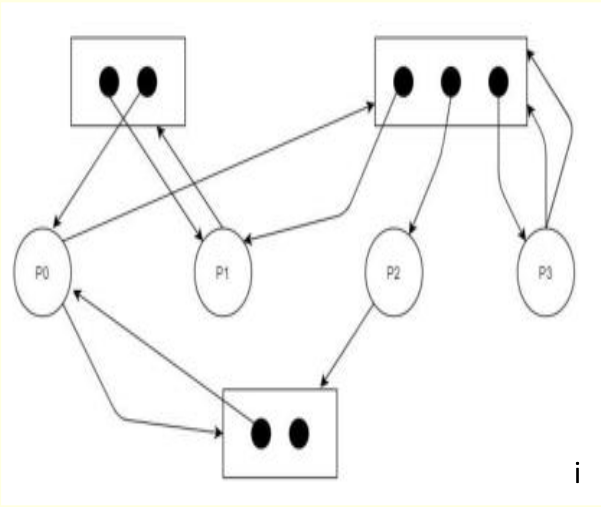
\includegraphics[width=\textwidth]{pics/img1.png}
		\caption{گراف ۱}
		\label{شکل۱ الف}
	\end{subfigure}
	\hfill
	\begin{subfigure}[b]{0.3\textwidth}
		\centering
		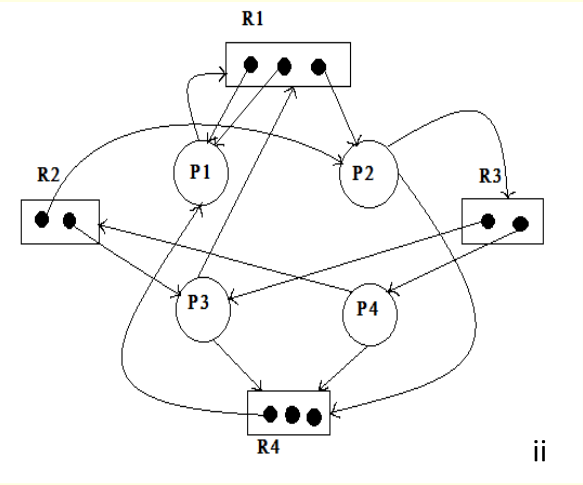
\includegraphics[width=\textwidth]{pics/img2.png}
		\caption{گراف ۲}
		\label{شکل۱ ب}
	\end{subfigure}
	\hfill
	\begin{subfigure}[b]{0.3\textwidth}
		\centering
		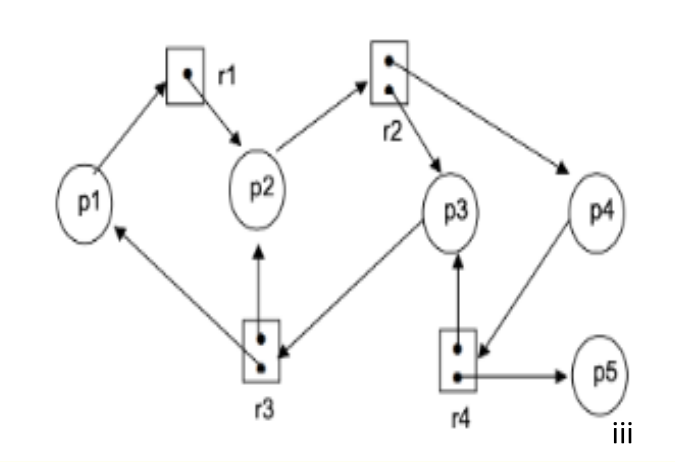
\includegraphics[width=\textwidth]{pics/img3.png}
		\caption{گراف ۳}
		\label{شکل۱ ج}
	\end{subfigure}
	\caption{گراف‌ها}
	\label{شکل ۱}
\end{figure}








	
%\begin{figure}[htbp]
%	\centering
%	\begin{tikzpicture}
%		% Draw circles with labels
%		\draw (0,0) circle (0.5) node (p0) {$p_0$};
%		\draw (2,0) circle (0.5) node (p1) {$p_1$};
%		\draw (4,0) circle (0.5) node (p2) {$p_2$};
%		\draw (6,0) circle (0.5) node (p3) {$p_3$};
%		
%		% Draw rectangles above circles
%		\draw (0,1) rectangle (2,2);
%		\draw (4,1) rectangle (6,2);
%		
%		% Draw circles inside the first rectangle (colored in black)
%		\draw[fill=black] (0.5,1.5) circle (0.2);
%		\draw[fill=black] (1.5,1.5) circle (0.2);
%		
%		% Draw circles inside the second rectangle (colored in black)
%		\draw[fill=black] (4.5,1.5) circle (0.2);
%		\draw[fill=black] (5,1.5) circle (0.2);
%		\draw[fill=black] (5.5,1.5) circle (0.2);
%		
%		% Draw rectangle below circles
%		\draw (2,-1) rectangle (4,-2);
%		
%		% Draw circles inside the third rectangle (colored in black)
%		\draw[fill=black] (2.5,-1.5) circle (0.2);
%		\draw[fill=black] (3.5,-1.5) circle (0.2);
%		
%		% Draw dashed arrows
%		\draw[->, solid] (1.6,1.5) -- (p0);
%		\draw[->, solid] (2.3,-1.5) -- (p0);
%		\draw[->, solid] (0.5,1.5) -- (p1);
%		
%		
%		
%		
%		
%		
%		\draw[->, solid] (p0) -- (2,-1);
%		\draw[->, solid] (p0) -- (4,1.8);
%		\draw[->, solid] (p1) -- (1.6,1);
%	\end{tikzpicture}
%	\caption{الف}
%	\label{fig:resource-allocation-graph}
%\end{figure}

